\documentclass[10pt]{article}
\usepackage[margin=17mm]{geometry}
\usepackage{graphicx,booktabs,hyperref}
\usepackage[strings]{underscore}
\setlength{\parindent}{0pt}\setlength{\parskip}{5pt}
\begin{document}
\section*{Fresh fixtures: target lifts on the E0 reference curve}
Native correctness/relevance run, 2026-10-25. All 1,152 frozen targets
across 36 files, nine parameter cells and four families are retained.
E0 is $y^2+xy=x^3+1$ over each input's exact GF($2^n$) representation.
The Boolean solution count is copied from the frozen fixture, not recomputed
by this audit. Complete y-root solving, substitution and an independent
Artin--Schreier trace criterion agree for every target.

\begin{center}\begin{tabular}{lrr}\toprule
Frozen Boolean class & E0 lift & No E0 lift\\\midrule
SAT & 154 & 176\\
UNSAT & 434 & 388\\
\bottomrule\end{tabular}\end{center}
\begin{center}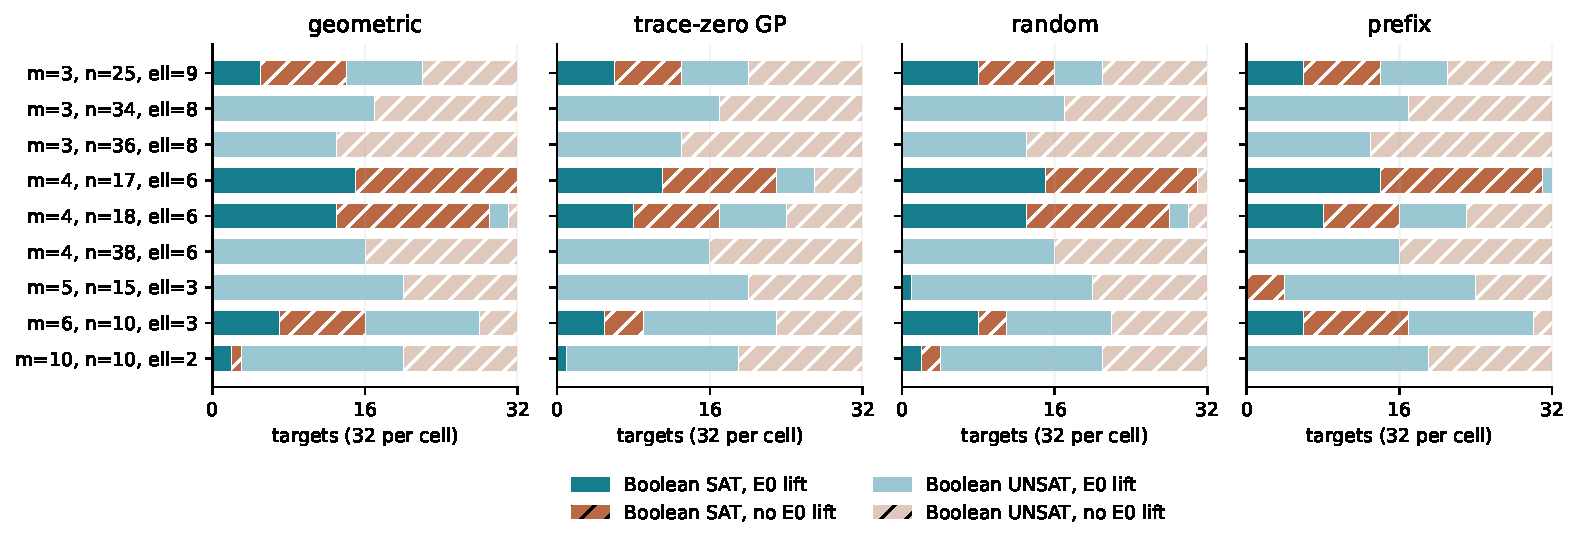
\includegraphics[width=\linewidth]{target-lift-classes.pdf}\end{center}

\textbf{Scope.} These are x-only Boolean fixtures. They do not specify a
full curve coefficient a, group order or subgroup. The b=1 S3 equation is
independent of a. This audit explicitly chooses a=0 as its reference model;
``no E0 lift'' is not invalidity for every b=1 curve or twist. A positive E0
lift establishes neither subgroup membership nor a signed factor-base point
decomposition. The uniform field-x target law is not an ordinary subgroup
query law. Preserve all four classes; do not silently filter them or
retrofit a different experiment.

\textbf{Consequence.} The closure panels and guess branches remain finite
algebraic evidence. Their relevance to ordinary IC relation generation
needs separate curve/subgroup-qualified inputs, complete lifting and
relation verification. No degree bound, security exponent, speed or cost
improvement follows from this diagnostic.

Frozen audit source: c3b2bd27d, \path{examples/ic_fresh_relevance.rs}.
The command is \path{ic_fresh_relevance inputs/fresh}; protocol:
\path{../../FRESH_RELEVANCE_PROTOCOL.md}. Local shared x86-64 host, L0,
12-GiB address-space limit and 900-second process limit; exit 0. The complete
JSON binds all 36 input files by SHA-256 and retains every target and y root.
A second native execution is byte-identical. This is a deterministic rerun,
with independent trace checking inside the auditor, not an external
large-cell solver replay or hardware measurement.

Receipt: \path{../../pipeline-receipts/fresh-target-relevance-20261025/receipt.json}.
Source/binary hashes, status, times and replay comparison accompany it.
\end{document}
